\documentclass[12pt]{article}
\usepackage[T1]{fontenc}
\usepackage{graphicx}
\usepackage[table,xcdraw]{xcolor}
\usepackage{enumerate}
\usepackage{lipsum}
\usepackage[final]{pdfpages}
\usepackage[toc,page]{appendix}
\usepackage{verbatimbox}
\usepackage{multirow}
\usepackage[ruled,linesnumbered]{algorithm2e}
\usepackage[english,brazil]{babel}
\usepackage{soul}
\usepackage{pgfgantt}

\usepackage[style=abnt]{biblatex}
\addbibresource{referencias.bib}

\usepackage{longtable}
\usepackage{colortbl}%
   \newcommand{\myrowcolour}{\rowcolor[gray]{0.925}}

% \usepackage{pgfgantt}

% \usepackage{listings,xcolor}
% \lstset{
%     string=[s]{"}{"},
%     stringstyle=\color{blue},
%     comment=[l]{:},
%     commentstyle=\color{black},
% }

\usepackage{hyperref}
\hypersetup{
    colorlinks=true,
    linkcolor=blue,
    filecolor=magenta,      
    urlcolor=cyan,
}

\usepackage{tikz}
\usepackage{calc}
\usepackage{booktabs}
\usepackage{caption}
\usepackage[table,xcdraw]{xcolor}


% colors
\definecolor{color1}{HTML}{b30000}
%\definecolor{color1}{HTML}{8C260F}
\definecolor{color2}{HTML}{333333}


% fonts
\usepackage{fontspec}
\defaultfontfeatures{Mapping=tex-text}
\setmainfont
[BoldFont=Lato-Bold.ttf,
ItalicFont=Lato-Italic.ttf,
BoldItalicFont=Lato-BoldItalic.ttf]
{Lato-Regular.ttf}
\newfontfamily\headingfont[ItalicFont=Lato-BlackItalic.ttf]{Lato-Black.ttf}
%%%

\usepackage{geometry}
\geometry{a4paper,
hmargin=20mm,vmargin=20mm,
head=0ex,foot=3ex}

\linespread{1.3}

% \usepackage[hang]{caption}
%\DeclareCaptionFormat{upper}{#1#2\uppercase{#3}\par}
% \captionsetup{labelfont={bf,color=color2},textfont={normalsize,color=color2},format = upper,figurename=Figure,tablename=Table}

%%% fancy sections
\usepackage{titlesec}
%\titleformat{\chapter}{\headingfont\LARGE\bfseries\scshape\color{color1}}{\thechapter}{1em}{}[\titlerule]
\titleformat{\section}{\color{color1}\headingfont\Large\bfseries\uppercase}{\thesection}{1em}{}[\titlerule]
\titleformat{\subsection}{\color{color1}\headingfont\large\bfseries\uppercase}{\thesubsection}{1em}{}
\titleformat{\subsubsection}{\color{color1}\headingfont\bfseries\uppercase}{\thesubsubsection}{1em}{}
%%%

% head and foot
\usepackage{fancyhdr}
\pagestyle{fancy}
\makeatletter
\rhead{
\includegraphics[height=4ex]{ufpa_logo.png}}
\lhead{}
\makeatother
\newlength{\myheight}

\cfoot{\color{color2}FCT/ITEC/UFPA }
\rfoot{\color{color2}\thepage}
\renewcommand\headrulewidth{0pt}
\renewcommand\footrulewidth{0pt}

\usepackage{tabulary}
\usepackage{multirow}

% custom titlepage
\makeatletter
\newcommand*\DefVar[1]{\@namedef{#1}##1{\global\@namedef{get#1}{##1}}}
\DefVar{summary}
\renewcommand{\maketitle}{
\begin{center}
\begin{tikzpicture}
    \node[draw=none,%color1,line width=0.4pt,
      fill=color1,
      inner sep = 10pt,
      text width=\textwidth-20pt,
      text centered
    ] {\color{white}\headingfont\bfseries\huge Proposta de Projeto};
\end{tikzpicture}
\bigskip\bigskip\bigskip\\
% \includegraphics[width=\textwidth]{opening}\par
\headingfont\bfseries\Large Universidade Federal do Pará \\
Instituto de Tecnologia \\
Faculdade de Engenharia da Computação e Telecomunicações
\bigskip\bigskip\bigskip\bigskip\bigskip\bigskip\bigskip \\
\headingfont Projetos de Engenharia 3
\bigskip\bigskip\bigskip\bigskip\bigskip\bigskip\bigskip \\
{\color{color2}\normalfont\normalsize\textbf{}\\

\begin{table*}[htp]
\footnotesize
\centering
\begin{tabulary}{\linewidth}{|L|L|}
\hline
\begin{tabular}{l}\textbf{Documento}: \\ Projeto\end{tabular}
 &
\begin{tabular}{l}\textbf{Status}: \\ \color{red}PRIVADO\end{tabular}
\\ \hline
\begin{tabular}{l}\textbf{Disciplina}: \\
Projetos de Engenharia 3
\end{tabular}
&
\begin{tabular}{l}
\textbf{Data}: \\
\@date
\end{tabular}
\\ \hline
\end{tabulary}
\end{table*}

}
\end{center}
\clearpage
}
\makeatother
%%%

%%% fancy boxes
\usepackage{tcolorbox}
\usepackage{wrapfig}
\def\fullboxbegin{
\bigskip
\begin{tcolorbox}[colback=color1,colframe=color1,coltext=white,arc=0mm,boxrule=0pt]
}
\def\fullboxend{\end{tcolorbox}\medskip}
%
\def\leftboxbegin{
\begin{wrapfigure}{l}{0.5\textwidth}
\begin{tcolorbox}[colback=color1,colframe=color1,coltext=white,arc=0mm,boxrule=0pt]
}
\def\leftboxend{
\end{tcolorbox}
\end{wrapfigure}
}
%
\def\rightboxbegin{
\begin{wrapfigure}{r}{0.5\textwidth}
\begin{tcolorbox}[colback=color1,colframe=color1,coltext=white,arc=0mm,boxrule=0pt]
}
\def\rightboxend{
\end{tcolorbox}
\end{wrapfigure}
}
%
\newcounter{frames}
\def\frameboxbegin#1{
\bigskip
\refstepcounter{frames}
\begin{tcolorbox}[colback=white,colframe=color1,arc=0mm,title={\MakeUppercase{\textbf{Frame \arabic{frames}}: #1}}]
}
\def\frameboxend{
\end{tcolorbox}
}
%%%

\usepackage{lipsum}

%%%%%%%%%%%%%%%
% Title Page
\date{\today}
%%%%%%%%%%%%%%%

\begin{document}

\maketitle

\tableofcontents
\newpage

\section{Identificação}
\label{sec:ident}
\textcolor{red}{Leiam com atenção as partes em vermelho!}
\textcolor{red}{ 
\begin{enumerate}
    \item As partes em vermelho fornecem uma breve explicação do modelo de proposta do projeto. 
    \item Os discentes devem remover as partes em vermelho na versão final!
    \item Esse modelo deve ser usado como uma \textbf{ferramenta de planejamento}, portanto, faz parte do projeto de vocês. Planos podem sofrer modificações durante a execução do projeto, contudo uma boa execução depende de um bom plano prévio ao início das atividades de execução do projeto. \textbf{Um bom projeto começa com um bom planejamento}!
    \item Em cada parte, o grupo pode ter flexibilidade para escrever de maneira diferente do que  está sugerido, mas combine com o professor.
\end{enumerate}
}

\subsection{Título do Projeto}

\textcolor{red}{Por exemplo: Projeto de radar de velocidade de carros de baixo custo para ambientes privados.} 

\subsection{Profissionais e entidade(s) participantes}

\textcolor{red}{Relação dos nomes dos participantes do projeto. Incluam o nome e matrícula. Sugestão: procurem também incluir possíveis laboratórios envolvidos, empresas e demais ambientes de execução do projeto.}

\textcolor{red}{\textit{Por exemplo, Fulana (matrícula XXXXXX), Cicrano (matrícula YYYYYYY) e  Beltrano (matríicula ZZZZZZ) serão responsáveis pela execução do projeto sob a tutoria do prof. QQQQQ. Parte do desenvolvimento será realizado no laboratório XXXX, na empresa YYY e nas acomodações de VVVVVVV.}}

\newpage
\section{Introdução}
\label{sec:intro}
\subsection{Problema abordado}
\label{sec:problema}

\textcolor{red}{Descrição do problema a ser resolvido, uma condição a ser aprimorada ou produto desenvolvido.}

\textcolor{red}{Procure justificar seu problema com clareza, trazendo dados sobre a importância dele e sobre a necessidade das pessoas para que seja resolvido. Um problema bem definido  precisa ser:
\begin{itemize}
    \item Escrito em termos humanos (ao invés de tecnologia, produto ou funcionalidade de serviço);
    \item Abrangente o suficiente para permitir que você descubra áreas de valor inesperado;
    \item Específico o suficiente para ser gerenciável;
    \item Em formato de pergunta começando com “Como podemos..."
\end{itemize}}

\textcolor{red}{Procure ainda posicionar o problema em relação às diretrizes municipais, estaduais, nacionais e/ou mundiais. Exemplo: o problema está relacionado com uma das metas da ONU? o problema está previsto no plano diretor de uma secretaria de estado?}

\textcolor{red}{\textit{Por exemplo, desenvolvimento de um sistema de radar de carros que monitorem a velocidade dos carros em estacionamentos, pequenas vilas ou locais onde os carros tenham um limite de velocidade preestabelecido. (Este exemplo é bem sucinto e o grupo pode descrever mais aqui. Um problema claramente descrito significa menos dor de cabeça na execução do projeto! O escopo do  problema é definido principalmente nesta seção).}}

\textcolor{red}{
Nesta seção você deve ter referências dando suporte ao seus argumentos. Para citar, inclua o bibtex do material que deseja citar no arquivo "referencias.bib" e use o comando "cite" da forma que fazemos a seguir \cite{lee2020deep}. Neste sentido é importante lembrar que um projeto é um documento focado e que nele não há espaço para uma seção de bibliografia (geralmente comum em textos mais longos como livros), mas apenas podemos colocar referências bibliográficas, que coletam aqueles materiais que foram efetivamente usados ao longo do texto.}

\textcolor{red}{Notas de rodapé podem ser usadas para indicar comentários ou um site, por exemplo.\footnote{\url{http://www.ufpa.br}}}

\textcolor{red}{Nesta seção, você pode trazer figuras e tabelas para ilustrar o problema. A Figura \ref{fig:exemplo} e a Tabela \ref{tab:exemplo} mostram como fazer isso. Use estes \textit{templates} para adicionar outras figuras e tabelas.}

\begin{figure}[ht]
\centering
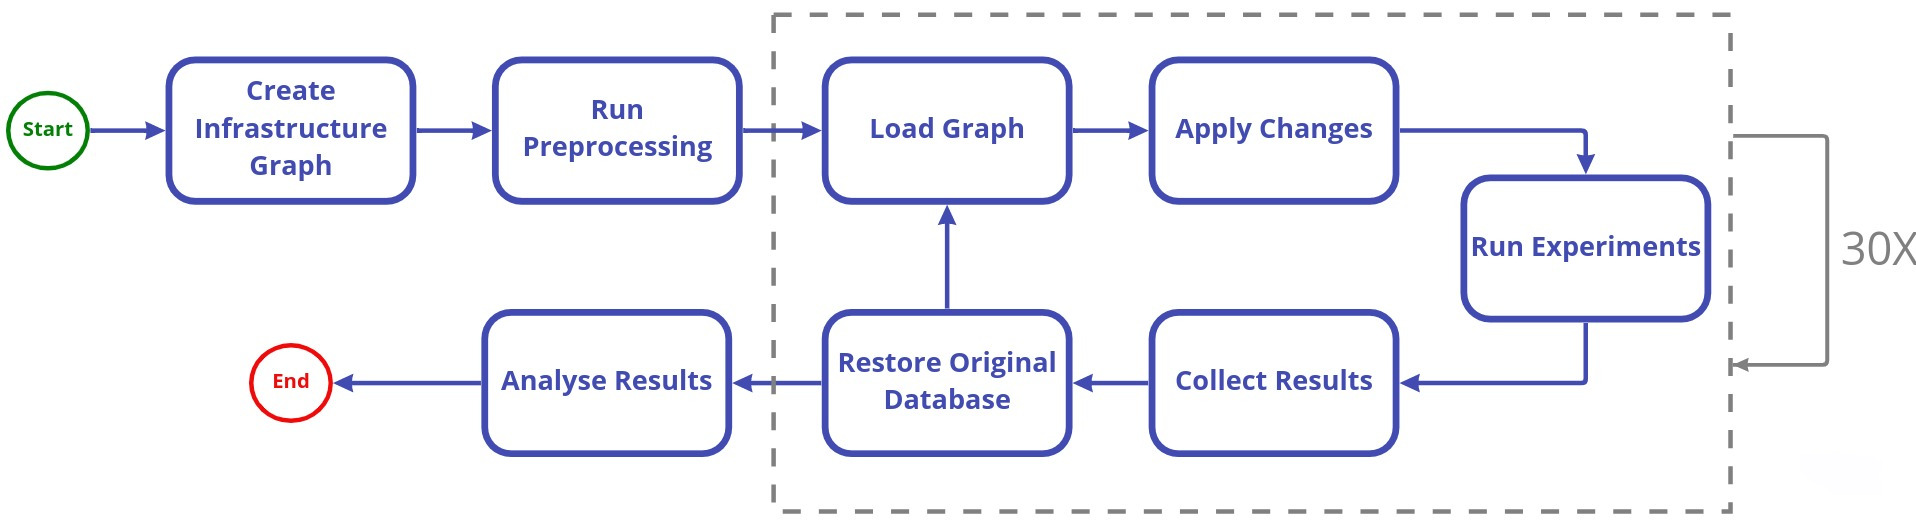
\includegraphics[width=0.9\textwidth]{figures/methodology.jpg}
\caption{Figura de exemplo}
\label{fig:exemplo}
\end{figure}


\begin{table}[ht]
\centering
\caption{Tabela de exemplo}
\label{tab:exemplo}
\begin{tabular}{@{}cc@{}}
\toprule
\textbf{Factors}                       & \textbf{Levels}          \\ \midrule
Heuristic levels                       & 1 and 2                  \\
Graph size                             & 1,000, 5,000, and 10,000 \\
Subgraph type                          & Inter and intra          \\
Elements to be added/disabled           & Nodes and Links          \\
Number of elements to be added/disabled & 1, 5, 10                \\ \bottomrule
\end{tabular}
\end{table}

\textcolor{red}{Um ponto importante sobre figuras e tabelas em textos técnicos é que uma figura nunca deve ser colocada se não houver algo para dizer sobre ela. Então antes de adicionar a figura procure pensar sobre o que você quer que o leitor veja nela? qual argumento ela vai lhe ajudar a compor? Procure não adicionar figuras que sejam meramente ilustrativas}

\subsection{Objetivo Geral}

\textcolor{red}{O objetivo indica o que o projeto quer alcançar no mais alto nível, de forma clara e em uma frase. O formato típico de um objetivo estratégico é "Verbo + Adjetivo + Substantivo". Ao seguir esse formato, teremos a criação de uma declaração de ação. Um projeto grande pode ter mais de um objetivo, mas para o contexto desta disciplina basta um que seja claro.}

\textcolor{red}{\textit{Por exemplo, promover um melhor monitoramento da velocidade dos carros, de maneira a notificar usuários que ultrapassem o limite pré-estabelecido de velocidade em estacionamento privativos como em condomínios ou vilas, onde acidentes podem ocorrer com crianças ou animais.}}

\textcolor{red}{Nesta seção você pode explicar a solução pensada e justificá-la frente ao problema proposto. Procure então adicionar dados, argumentos e referências que mostrem que esta solução é adequada e viável. Procure ainda descrever outras soluções para o mesmo problema.}

\textcolor{red}{Aqui você deve também associar seu projeto aos requisitos da disciplina, de modo a justificar que ele se encaixa no que é pedido pelo professor.}

\subsection{Objetivo Específico}

\textcolor{red}{Objetivos específicos representam o desdobramento dos objetivos gerais em partes menores. Representam os objetivos para os quais o projeto trabalha para alcançá-los dentro de um prazo estipulado. Eles devem abordar diretamente o problema mencionado na Declaração do Problema. Um projeto de disciplina não deveria ter mais que dois ou três destes.}

\textcolor{red}{\textit{Por exemplo, construção de sistemas de monitoramento de velocidade de veículos que seja de baixo custo.}}

\subsection{Duração do Projeto}

\textcolor{red}{Indique a duração do projeto em semanas. Tenha em mente o cronograma da disciplina na hora de preencher esta seção. Considere os momentos de apresentação mais gerais e as datas previstas para as entregas.}

\newpage
\section{Plano de Execução}
\label{sec:plano}
\subsection{Materiais e Métodos}

\textcolor{red}{Aqui deve-se informar como a equipe pretende executar o projeto. Algumas perguntas que deveriam estar respondidas nesta seção são: “Quais os conjuntos de passos que serão usados para o desenvolvimento do projeto?”, “Qual a organização sistemática das ações?”, “Como a equipe pretende avaliar o andamento do projeto continuamente (reuniões periódicas, por e-mail, grupo de e-mail, etc)?”, }

\textcolor{red}{Certamente, no momento da escrita deste documento a equipe ainda possuirá um bom número de dúvidas à respeito de como o projeto será executado. Contudo, o planejamento serve exatamente para remover estas dúvidas. Procure antecipar o máximo das decisões. Exemplo, se vai usar um certo conjunto de dados, procure definir e explicar, em detalhes, quais as características deste conjunto de dados. Se vai usar uma API, explique como ela funciona e como se encaixará no projeto.}

\textcolor{red}{As escolhas de métodos e materiais devem vir acompanhadas de justificativas. Por que você pretende usar uma plataforma de prototipação de hardware Y e não a X? Ou porque você pretende usar a linguagem de programação X e não Y}

\textcolor{red}{Atente-se que esta seção não é desligada da Seção \ref{sec:problema}, portanto tente encadeá-la de modo a mostrar que o método levará ao desenvolvimento da solução.}

\textcolor{red}{Em alguns casos, talvez você já saiba que vai empregar determinado algoritmo. Então você pode documentá-lo nesta seção da seguinte forma. Como no Algoritmo \ref{alg:level0}.}

\begin{algorithm}[hbt!]
\caption{Level 0 update}\label{alg:level0}
\KwData{The VNF list and flow entry list to be placed}
\KwResult{Update the network}

\For{each VNF}{
update physical node capacity according to requirements of the VNF that was placed at it
\label{line:update-resources-nodes}

store information in database
}

\For{each flow entry}{
update physical link capacity according to the bandwidth requirements of the flow entry that was just placed
\label{line:update-resources-links}

store information in database
}
\end{algorithm}

\textcolor{red}{Lembre-se que você deve comentar qualquer artefato que venha a adicionar no texto seja uma figura, tabela ou algoritmo. Se quiser, no caso dos algoritmos, pode inclusive referenciar linhas, como as linhas \ref{line:update-resources-nodes} e \ref{line:update-resources-links}.}

\subsection{Escopo e \textit{Work Packages}}

\textcolor{red}{Para o desenho do Escopo é sugerido que o primeiro passo seja definir as entregas criando a Estrutura Analítica do Projeto (EAP), também conhecida pelo termo em inglês, \textit{Work Breakdown Structure} (WBS). Uma EAP é um processo de subdivisão das entregas e do trabalho do projeto em componentes menores e mais facilmente gerenciáveis, geralmente chamados de módulos, pacotes de trabalho, ou \textit{Work Packages}. É útil para alinhar o entendimento do projeto e integrar todas as áreas.}

\textcolor{red}{O foco básico de um pacote de trabalho ou atividade é nas entregas. Qual o artefato esperado nesta atividade? E neste pacote de trabalho, o que esperamos construir nele? Artefatos podem ser relatórios, vídeos, código, esquemas, circuitos etc. Tenha isso em mente conforme determina as atividades de seu projeto.}

\textcolor{red}{A EAP deve ser completa, organizada e subdivida o suficiente para tornar possível a medição do progresso, mas não detalhada o suficiente para se tornar, ela mesma, um obstáculo à realização do projeto.}

\textcolor{red}{Cada WP deve ter um objetivo claro, atividades e entregáveis bem definidos. A partir da definição dos objetivos e entregáveis, é necessário estabelecer as atividades necessárias de cada WP para realizá-las.}

\textcolor{red}{Abaixo oferecemos exemplos de WPs para o caso do radar.}

\begin{longtable}{p{\textwidth}}
% pairs: absolute number (percentage)
\toprule%
\myrowcolour%
\bfseries WP1: Avaliação preliminar e compra de materiais \\
\midrule
\textbf{Objetivo}: Avaliar formas de monitorar a velocidade com auxílio de sinalizadores e captura de imagens. Após a análise preliminar, pretende-se comprar os componentes necessários para implementação dos algoritmos e sistemas propostos.\\
\midrule
\myrowcolour%
\bfseries Entregáveis \\
\midrule
\textbf{E1.1}: lista de algoritmos e sistemas para implementar o produto proposto. \\
\textbf{E1.2}: lista de materiais necessários e sistemas para implementar o produto proposto. \\
\midrule
\myrowcolour%
\bfseries Atividades \\
\midrule
\textbf{A1.1}: Ler artigos, livros, blogs…. Para entender os detalhes para implementação do sistemas. \\
\textbf{A1.2}: Buscar materiais necessários para implementação do sistema. \\
\bottomrule
\end{longtable}

\begin{longtable}{p{\textwidth}}
% pairs: absolute number (percentage)
\toprule%
\myrowcolour%
\bfseries WP2: Interface com a câmera \\
\midrule
\textbf{Objetivo}: Entender como capturar as imagens de câmeras e entregá-las para um outro software processá-la.\\
\midrule
\myrowcolour%
\bfseries Entregáveis \\
\midrule
\textbf{E2}: software ou biblioteca que permita a leitura de imagens da câmera. \\
\midrule
\myrowcolour%
\bfseries Atividades \\
\midrule
\textbf{A2.1}: Ler documentação da câmera\\
\textbf{A2.2}: Construir código para receber dados da câmera\\
\bottomrule
\end{longtable}

\begin{longtable}{p{\textwidth}}
% pairs: absolute number (percentage)
\toprule%
\myrowcolour%
\bfseries WP3: Implementação do sistema de monitoramento de velocidade \\
\midrule
\textbf{Objetivo}: Implementação dos algoritmos.\\
\midrule
\myrowcolour%
\bfseries Entregáveis \\
\midrule
\textbf{E3}: Sistema que calcula a velocidade dos carros com base no sistema de monitoramento. \\
\midrule
\myrowcolour%
\bfseries Atividades \\
\midrule
\textbf{A3.1}: Desenvolvimento de sistema de captura de velocidade dos carros.\\
\bottomrule
\end{longtable}

\begin{longtable}{p{\textwidth}}
% pairs: absolute number (percentage)
\toprule%
\myrowcolour%
\bfseries WP4: Acompanhamento, Integração, Instalação e testes em campo \\
\midrule
\textbf{Objetivo}: Integração de todas as partes do sistema e montagem em campo para realização de testes e eventuais ajustes.\\
\midrule
\myrowcolour%
\bfseries Entregáveis \\
\midrule
\textbf{E4.1}: Sistema funcionando. \\
\textbf{E4.2}: Relatório técnico descrevendo o sistema proposto. \\
\midrule
\myrowcolour%
\bfseries Atividades \\
\midrule
\textbf{A4.1}: Acompanhamento e integração de todos os sistemas \\
\textbf{A4.2}: Desenvolvimento de interface gráfica amigável para visualização dos dados monitorados \\
\textbf{A4.3}: Escrita de relatório técnico descrevendo o sistema desenvolvido.\\
\bottomrule
\end{longtable}

\subsection{Cronograma}
\textcolor{red}{Um cronograma de atividades deve ser estimado, a partir das atividades planejadas para cada work package. O cronograma deve estimar um tempo para cada atividade e seus pré-requisitos. A primeira etapa do cronograma é o planejamento e deve constar no cronograma.}

\textcolor{red}{O cronograma também deve conter as datas das entregas de cada entregável.}

\textcolor{red}{Abaixo oferecemos exemplo de um cronograma para o caso do radar. Observe que, neste caso, fazemos uso dos códigos que criamos anteriormente. O calendário está em semanas e os números abaixo dos meses indicam o dia do mês em que a semana começa.}

\ganttset{%
    calendar week text={%
        \startday
    }%
}

\begin{ganttchart}[
  hgrid,
  vgrid,
  x unit=0.20cm,
  time slot format=isodate,
  bar height=0.5,
  inline,
  bar/.append style={fill=gray!50, inner sep=0pt}
  ]{2022-09-19}{2022-12-09}
\gantttitlecalendar{year, month=name, week=1} \\

\ganttbar{A1.1}{2022-09-19}{2022-10-16} 
\ganttmilestone{E1.1}{2022-10-09} \\
\ganttbar{A1.2}{2022-09-26}{2022-10-09} 
\ganttmilestone{E1.2}{2022-10-09} \\
\ganttbar{A2.1}{2022-10-03}{2022-10-30} \\
\ganttbar{A2.2}{2022-10-17}{2022-11-06} 
\ganttmilestone{E2}{2022-10-31} \\
\ganttbar{A3.1}{2022-10-24}{2022-11-20} 
\ganttmilestone{E3}{2022-11-20} \\
\ganttbar{A4.1}{2022-09-19}{2022-12-09} 
\ganttmilestone{E4.1}{2022-11-28} \\
\ganttbar{A4.2}{2022-11-14}{2022-12-09}
\ganttmilestone{E4.2}{2022-12-05} \\

\end{ganttchart}

\newpage

\textcolor{red}{Todo projeto de uma solução parte de conhecimento prévio para geração de algo novo, ou seja, todo projeto deveria ter um bom número de referências que apoiem a proposta. Referências podem ser artigos científicos e matérias de jornais que tragam dados que subsidiem o problema. Pode-se ainda citar artigos científicos que ilustrem o método a ser utilizado no desenvolvimento do projeto.}
\printbibliography


\end{document}
